\label{sec:background}

***************To Move to the introduction
In recent years, the increasing workload and demand of processing power in modern embedded systems paved the ground for multicore platforms to be commonly adopted.

Multicore can provide enormously larger processing capacity compared to the classical single core platforms,  so that larger systems can be deployed. However. ..complexity and predictability. ...

***********

This section introduces the scheduling fundamentals of shared resources in multicore platforms: cores, shared caches and DRAM. 

\begin{figure}[ht!]
\caption{Simplified multicore system architecture.}
\label{fig:architecture}
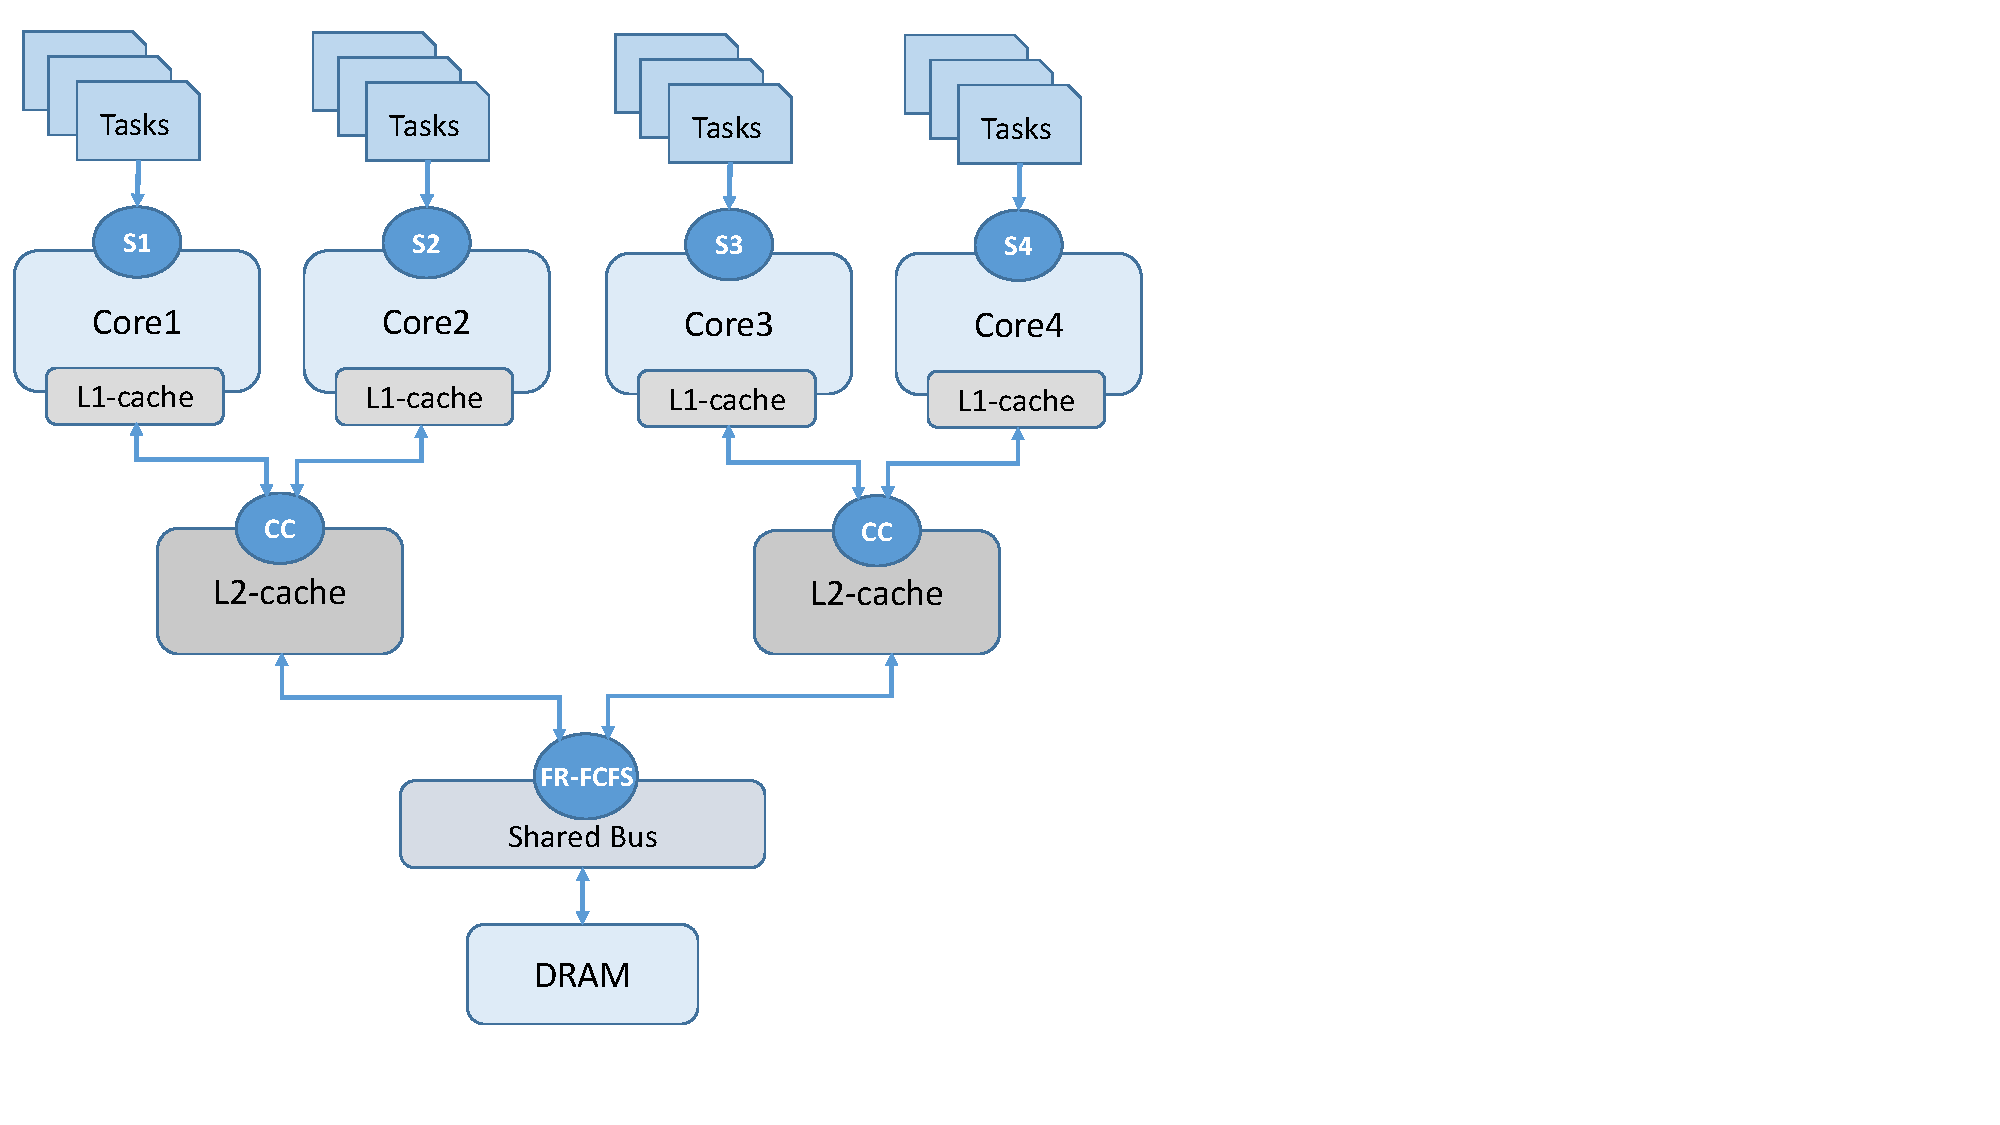
\includegraphics[scale=0.45]{architecture.pdf}
\end{figure}

The overall system architecture we consider in this paper is depicted in Figure~\ref{fig:architecture}, where is the cache coloring policy and $s_i$ are CPU scheduling policies.

\subsection{Cores Scheduling}
To leverage the processing performance of a computing system, a processing unit (core in our context) can be assigned more than one task, however only one task can execute effectively at any point in time. The arbitration between the different tasks execution is performed according to a scheduling policy. 

Basically, a scheduling policy determines, at any point in time, which task from the ready queue must execute first and when a given task can be preempted by another. Such a ready queue can be either local for a given core (Local scheduling) or common for a set of cores (Global Scheduling). The most commonly used scheduling algorithms are {Earliest Deadline First} (EDF), {Fixed Priority Scheduling} (FPS) and {Rate Monotonic} (RM).
The decision of selecting a task is made by the adopted scheduling algorithm while considering the whole task set configuration e.g.  the preemption attribute, static priorities or dynamic, etc. The key factor can be associated to the priority, remaining execution time or how far the deadline is.   
 
Another recent alternative to schedule memory intensive application tasks on a given core is the use of a memory-centric policy \cite{Yao2015,Yao2012}, where tasks are sorted in the queue according to a decreasing order of their numbers of memory requests.
In our setting, we are adopting FIFO, FPS and XXX as scheduling policies for the individual cores.    

\subsection{L2-Cache Scheduling}
In order to enhance the processing performance of multicore platforms, some of modern multicore processors \footnote{E.g. {Intel Core i7, AMD FX, ARM Cortex and FreeScale QorIQ} processors.} consider a shared cache level. The primary goal of sharing a cache level between different cores is to reduce the access requests to the main memory DRAM, and by that shorten the interference time due to DRAM access since the interference time is strongly correlated to the number of access requests \cite{Nowotsch14}. On the other hand, uncontrolled share of cache can lead to a degradation of performance and  predictability where starvation and data unconsistency can raise. To make the access to a shared cache manageable, an appropriate scheduling algorithm is primordial.

Cache coloring policy \cite{Hyoseung13} has been defined as an algorithm to schedule the access to the shared cache level L2.  
Essentially, it ***
 
\subsection{DRAM access Scheduling} 
Conventionally, a DRAM memory is usually shared by all the platform processing units in order to reduce the design cost. However, on the other hand, this increases the complexity of managing memory access and efficiency, in particular for multicore systems.  
To exploit efficiently the shared DRAMs, memory controllers have adopted scheduling mechanisms in a similar way as processors scheduling.

\begin{figure}[ht!]
%\vspace{-0.5cm}
\caption{Detailed DRAM architecture from \cite{Kim14}.}
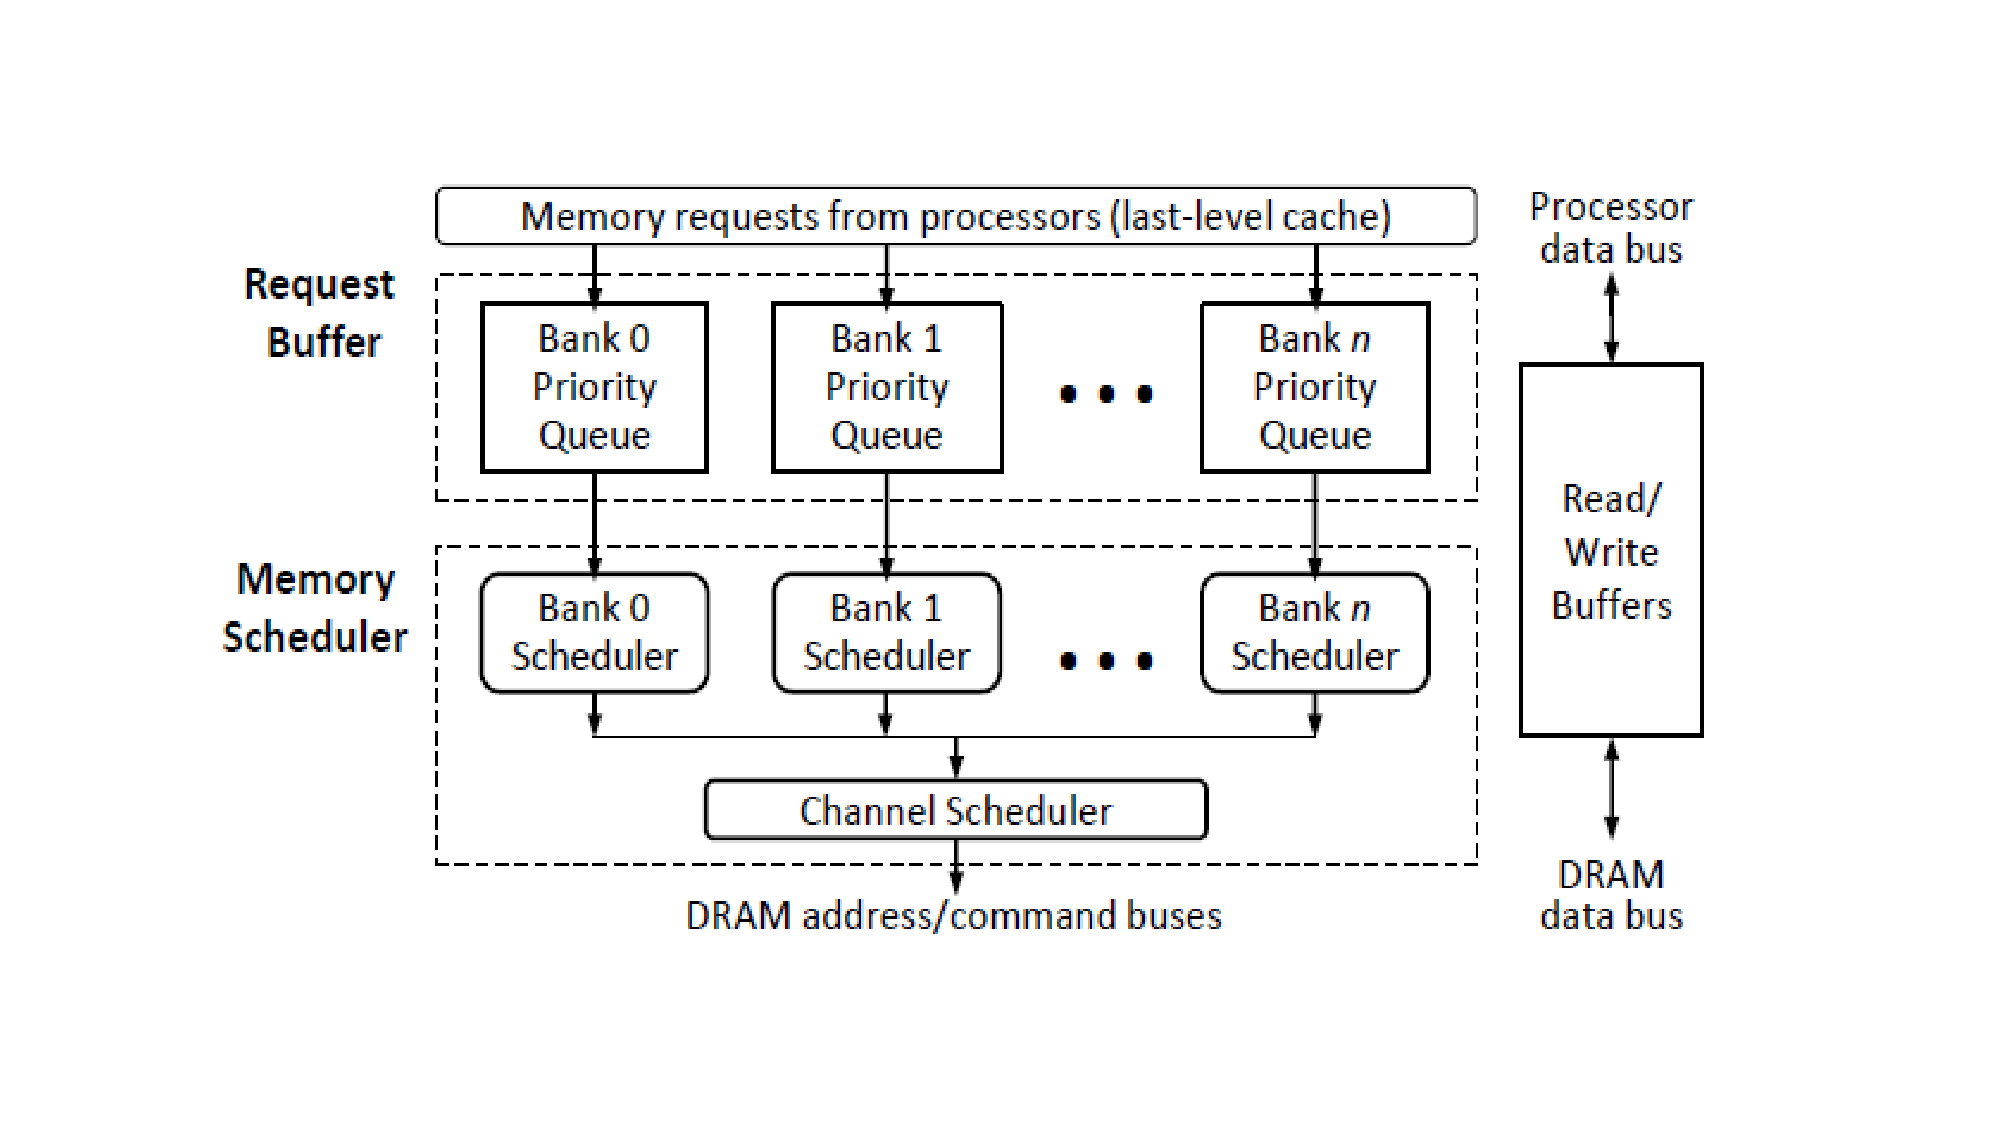
\includegraphics[scale=0.55]{dram-architecture.pdf}
\end{figure}

Naive conventional policies like {First Come First Served} (FCFS) and {Read-First} schedule access requests according to their arrival times, with a special preference to read requests since they cause the processor to stall while write requests can normally be performed by write buffers. 
Another alternative to schedule access requests to the DRAM memory, having a three-dimensional structure (bank, row and column), is the {Hit-First} policy. 

  The Hit-First algorithm schedules row buffer hits before misses to reduce
the average memory access latency and improve the bandwidth
utilization \cite{Hong99,Rixner2000}, because request hitting in the row buffer
has shorter latency than a row buffer miss.

Least-Request. The least-request scheme assigns the
highest priority to the requests from the thread with the
fewest pending requests for systems with SMT processors
[A performance comparison of dram memory system optimizations for SMT processor05]. 
The rationale is that returning a request from
that thread is likely to release more waiting instructions dependent
on the request than returning a request from other
threads.

In {Time Division Multiple Access} (TDMA) policy \cite{tdma}, the DRAM controller allocates statically a time slot to each core to access the DRAM in a circular manner, i.e. Round-Robin way. TDMA provides a simple and fair scheduling among all cores, however, it does not exploit the spatial locality available in memory access streams as it does not consider the demands coming from different programs at any time point.

To maximize data throughput and minimize the DRAM latency, memory controllers in modern COTS-based systems use {First Ready-First Come First Serve} (FR-FCFS) as a policy to schedule DRAM access requests \cite{Rixner2000,Nesbit2006,Kim14}.  FR-FCFS considers a detailed architecture of the memory structured in terms of banks, rows and columns. The DRAM scheduler can be viewed as a 2-level hierarchy: bank level and bus level. The access requests can target different banks separately, where they will be queued each in the corresponding bank queue. Access requests will be sorted at each bank queue first according to their readiness, then the   candidates selected from bank level will be further sorted at bus level where only the earliest (one) request gains the access at a time, i.e. the first request showing up at bus level among the requests being selected by banks schedulers. The readiness of a request is given by whether it hits in the row-buffer or not. If no request hits the row-buffer, older requests are prioritized over younger ones. *********add the figure of detailed DRAM**************
